\documentclass[conference]{IEEEtran}
\IEEEoverridecommandlockouts
% The preceding line is only needed to identify funding in the first footnote. If that is unneeded, please comment it out.
%\usepackage{cite}
\usepackage[utf8]{inputenc}
\usepackage[english]{babel}
\usepackage{amsmath,amssymb,amsfonts}
\usepackage{algorithmic}
\usepackage{graphicx}
\usepackage{textcomp}
\usepackage{xcolor}
\usepackage[backend=biber, style=ieee]{biblatex}
\usepackage{tikz}
\usepackage{algorithm}
\usepackage{setspace}
\usepackage{xcolor}
\usepackage{graphicx}

\usetikzlibrary{positioning}
\addbibresource{cosc428.bib}
\graphicspath{ {./images/} }

\begin{document}

\title{
	Identification and Classification of Gambling Dice using Commodity Hardware
}

\author{
	\IEEEauthorblockN{Jesse Patrick Sheehan}
	\IEEEauthorblockA{
		\textit{Department of Electrical and Computer Engineering} \\
		\textit{University of Canterbury}\\
		Christchurch, New Zealand \\
		jps111@uclive.ac.nz
	}
}

\maketitle

\begin{abstract}
	This paper proposes a method to identify dice values using image processing and machine learning techniques.
	Prior research uses the pips of a die to determine its value, whereas the proposed method detects the outline of the die.
	Canny's edge detection and Suzuki's contour tracing algorithms were used to extract die faces from an image.
	A convolutional neural network was used to classify these die faces and to provide a probable number value.
	\textcolor{red}{Close the abstract by mentioning at least one result number (and hopefully a comparison with prior research results).}
\end{abstract}

\begin{IEEEkeywords}
	dice, gambling, computer vision, machine learning
\end{IEEEkeywords}

\section{Introduction}

Dice value detection is a valuable tool for the gaming industry.
Common image processing and feature detection techniques can be used to identify the position of dice.
Machine learning algoithms can be used to classify the value of the dice.
Consumer-grade hardware devices are now more capable of handling the processing requirements of such methods.
This article offers a simple method of detecting and classifying dice.

\section{Background}

% Rather than just a summary of prior related research, write a critical review - that is, mention limitations of any prior research/algorithms cited.

Prior research in this field have taken advantage of numerous methods.

The ``SORTE'' system was commissioned by the Portuguese Gaming Inspection Authorities for use in casinos \cite{Correia1995}.
It identified the locations of the pips on all dice and uses spatial locality to assign values to each.
However, this system required specific dice, a birds-eye view of the surface, and a careful ambient lighting setup.

The system designed by Lapanja, et al., detects dice values for a mechanical gambling machine \cite{Lapanjaa}.
It uses color difference to identify the pips and template matching to classify the value of each die.
This method requires a birds-eye view, a high-contrast background surface, and relies on hard-coded masks for classification.

The system devised by Huang \cite{Huang2008} uses a modified unsupervised gray clustering algorithm. 
However, it requires a birds-eye view, a high-contrast background, and the number of dice to be known in advance.

Finally, the method proposed by Chung \cite{Chung2009} uses the least distance criterion to classify die values.
This method detects the pips and then groups the pips into valid configurations based on the relative distance between each pip.
This method requires a birds-eye view and has only been tested on up to four dice.

All of these methods have been constrained by either the camera angle, the number of dice, or the background surface.

\section{Method}

Contrary to previous research, this method detects the outside of each dice first, then isolates each die and employs a CNN to classify the value.

\subsection{Image Pre-processing}

The image (figure \ref{fig:original}) is obtained from a source such as a file or video stream.
Some pre-processing (figure \ref{fig:pre-processing}) is performed to remove extraneous information:
\begin{enumerate}
	\item The image is converted to grayscale to make subsequent processing faster. 
	\item A binary threshold is performed. Pixel values below 160 are set to black, and the remainder, to white.
	\item A gaussian blur is applied to the image. A kernel size of 5 was used.
\end{enumerate}
\begin{figure}
	\centering
	\includegraphics[width=0.3\textwidth]{original}
	\caption{The original image from a webcam.}
	\label{fig:original}
\end{figure}
%\begin{figure}
%	\centering
%	\begin{tikzpicture}[
%		rectnode/.style={rectangle, draw=black!60, fill=black!5, very thick, minimum size=5mm},
%	]
%
%		% nodes
%		\node[rectnode]	(gray) 								{Grayscale};
%		\node[rectnode] (threshold) [below=of gray] 		{Threshold};
%		\node[rectnode] (blur)  	[below=of threshold] 	{Blur};
%
%		% lines
%		\draw[thick, ->] (gray.south) -- (threshold.north);
%		\draw[thick, ->] (threshold.south) -- (blur.north);
%
%	\end{tikzpicture}
%	\caption{The image pre-processing pipeline.}
%	\label{fig:pre-processing}
%\end{figure}

\subsection{Die Face Detection}
The image is now sufficiently clean of noise and feature detection can now take place.
Figure \ref{fig:feature-detection} shows the feature detection process.
\begin{enumerate}
	\item Edge detection using the Canny \cite{Canny1986} algorithm is used. % mention parameters
	\item Contours are then detected using the algorithm described by Suzuki, et al. \cite{Suzuki1985}.
	\item Contours are rejected if they don't have four points (i.e. are not quadrilateral).
	\item Contours are rejected if they are too large or too small.
	\item Contours are then filtered by their shape. The shape rejection filter (algorithm \ref{alg:shape-rejection}) will reject shapes that are not square enough.
\end{enumerate}
\begin{algorithm}
	\setstretch{1.35}
	\caption{The shape rejection filter as pseudocode.}
	\label{alg:shape-rejection}
	\begin{algorithmic}
		\REQUIRE $0 \leq \delta \leq 1$ be the acceptable error factor
		\REQUIRE $P_n$ be the set of points in the rectangle
		\STATE $E_{12} \leftarrow ||P_2 - P_1||$
		\STATE $E_{34} \leftarrow ||P_4 - P_3||$
		\STATE $\Delta = \frac{|E_{12} - E_{34}|}{\textnormal{max}(E_{12}, E_{34})}$
		\IF {$\Delta \leq \delta$} \RETURN \TRUE \ELSE \RETURN \FALSE \ENDIF
	\end{algorithmic}
\end{algorithm}
\begin{figure}
	\centering
	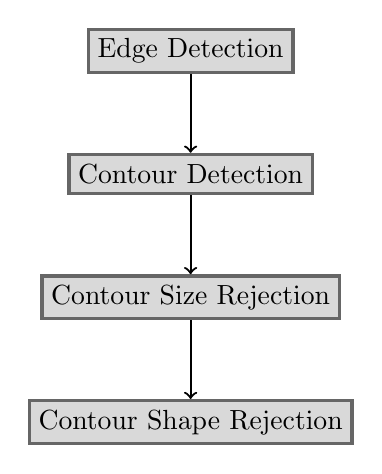
\begin{tikzpicture}[
		rectnode/.style={rectangle, draw=black!60, fill=black!15, very thick, minimum size=5mm},
	]
		
		% nodes
		\node[rectnode] (edge)							{Edge Detection};
		\node[rectnode] (contour) 	[below=of edge] 	{Contour Detection};
		\node[rectnode] (size)		[below=of contour] 	{Contour Size Rejection};
		\node[rectnode] (shape)		[below=of size]		{Contour Shape Rejection};

		% lines
		\draw[thick, ->] (edge.south) -- (contour.north);
		\draw[thick, ->] (contour.south) -- (size.north);
		\draw[thick, ->] (size.south) -- (shape.north);
	\end{tikzpicture}
	\caption{The image feature processing pipeline.}
	\label{fig:feature-detection}
\end{figure}

\subsection{Die Face Transformation}
The location and angle of the die face is now known within the original image.
Each die face must now be transformed before the CNN can be applied:
\begin{enumerate}
	\item Crop die face from the grayscale image obtained earlier.
	\item Rotate the image so that it lies flat against the vertical and horizontal axes.
	\item Scale the image so that it is 64 x 64 pixels (this is the image size that the CNN has been trained on).
	\item Apply the CNN model to the remaining image. This will produce a vector of probabilities that relate to each possible value (1 - 6).
	\item Select the most probable value. 
		If this value is below a specific threshold then the die cannot be classified.
		Otherwise, its value has likely been found.
\end{enumerate}

\subsection{Die Classification}

\section{Results}

\section{Conclusion}

\printbibliography

\end{document}
